\chapter{Experimental Design} \label{ch:Exp_Design}

\section{Testing Considerations}

\begin{wrapfigure}{r}{0.4\textwidth}
  \centering
    \includegraphics[width=0.4\textwidth]{whole_cart}
  \caption[Mobile Test Stand]{The mobile test stand, fully assembled. The aluminum rail holds the sensor mount 1~meter above the floor and is marked with an adhesive metric ruler for measuring camera displacement during PTAM initialization.}
  \label{fig:whole_cart}
\end{wrapfigure}

Before venturing further, we now summarize the goals of the UKF framework described previously, paying particular attention to the needs of unmanned aircraft system (UAS) operations. This ROS package was designed with the intent of producing estimates of the state of a rotorcraft UAV in real time. Thus, the experiments testing the system's efficacy compare the filter's estimates to the ground truth as measured by Vicon. Vicon, like many commercially available motion capture systems, works by using a number of infrared cameras (usually 8--12) to track the positions of retroreflector balls in the cameras' field of view. Each camera is outfitted with infrared LED\footnote{``Light-emitting diode,'' \url{https://en.wikipedia.org/wiki/Light-emitting_diode}} bulbs which illuminate the area with infrared light. The retroreflector balls reflect this infrared light back to the cameras, allowing the balls to be tracked as they move. Sets of these retroreflectors can be grouped together in software to represent rigid objects, allowing the Vicon system to track not only the position of an object, but its orientation as well.

\begin{figure}[t]
    \centering
    \begin{subfigure}[t]{0.5\textwidth}
        \centering
        \includegraphics[width=0.8\textwidth]{sensor_mount_top}
        \caption{Top view of sensor mount.}
    \end{subfigure}%
    ~ 
    \begin{subfigure}[t]{0.5\textwidth}
        \centering
        \includegraphics[width=0.8\textwidth]{sensor_mount_bottom}
        \caption{Bottom view of sensor mount.}
    \end{subfigure}
    \caption[3D-printed Sensor Mount]{The 3D-printed sensor mount. In (a), the Phidgets IMU is on the left and the mvBlueFOX camera is on the right. In (b), the linear braking handle and camera lens are visible.}
    \label{fig:sensor_mount}
\end{figure}

The UKF framework depends upon two sensors: a global-shutter monocular camera and an IMU. The IMU used in this experiment contains a 3-axis accelerometer and 3-axis gyroscope. To simulate both sensors moving through the scene in a manner reminiscent of hovering rotorcraft flight, a rolling test stand was constructed to carry the sensors safely throughout a large motion capture environment. Mounting the sensor suite (Figure~\ref{fig:sensor_mount}) on a large, steady, level platform (Figure~\ref{fig:whole_cart}) allows for a high degree of control over the accelerations and angular velocities felt by the IMU, as well as the motion captured by the ventral camera. In order to validate the UKF framework's effectiveness under ideal conditions, a modern laptop computer containing an Intel i7 processor with 16~GB of RAM\footnote{``Random-access memory,'' \url{https://en.wikipedia.org/wiki/Random-access_memory}} was used for all computations. The floor of the motion capture environment was strewn with a mixture of April tags and modified Quick Response\footnote{\url{https://en.wikipedia.org/wiki/QR_code}} (QR) codes in order to provide sufficient visual features for PTAM to track.

\subsection{PTAM Anomalies}

The experiments chosen to test the system's effectiveness were influenced largely by the known capabilities and limitations of the ROS PTAM implementation\footnote{From here on, ``PTAM'' refers to the particular ROS implementation of PTAM used in the experiments, not to the algorithm in general.}. In previous exploratory experiments\footnote{Performed both by the author and by various other parties at NASA Langley, where the experiments described here took place.}, PTAM was frequently shown to lose tracking\footnote{``Tracking'' here refers to current pose knowledge.} during large rotations. PTAM is particularly susceptible to losing tracking during \textit{pure} rotations, in which the camera rotates in place without translational motion. Worse, whenever PTAM undergoes a rotation, it interprets this as an arc-like motion, regardless of whether any translation took place.

\begin{wrapfigure}{r}{0.4\textwidth}
    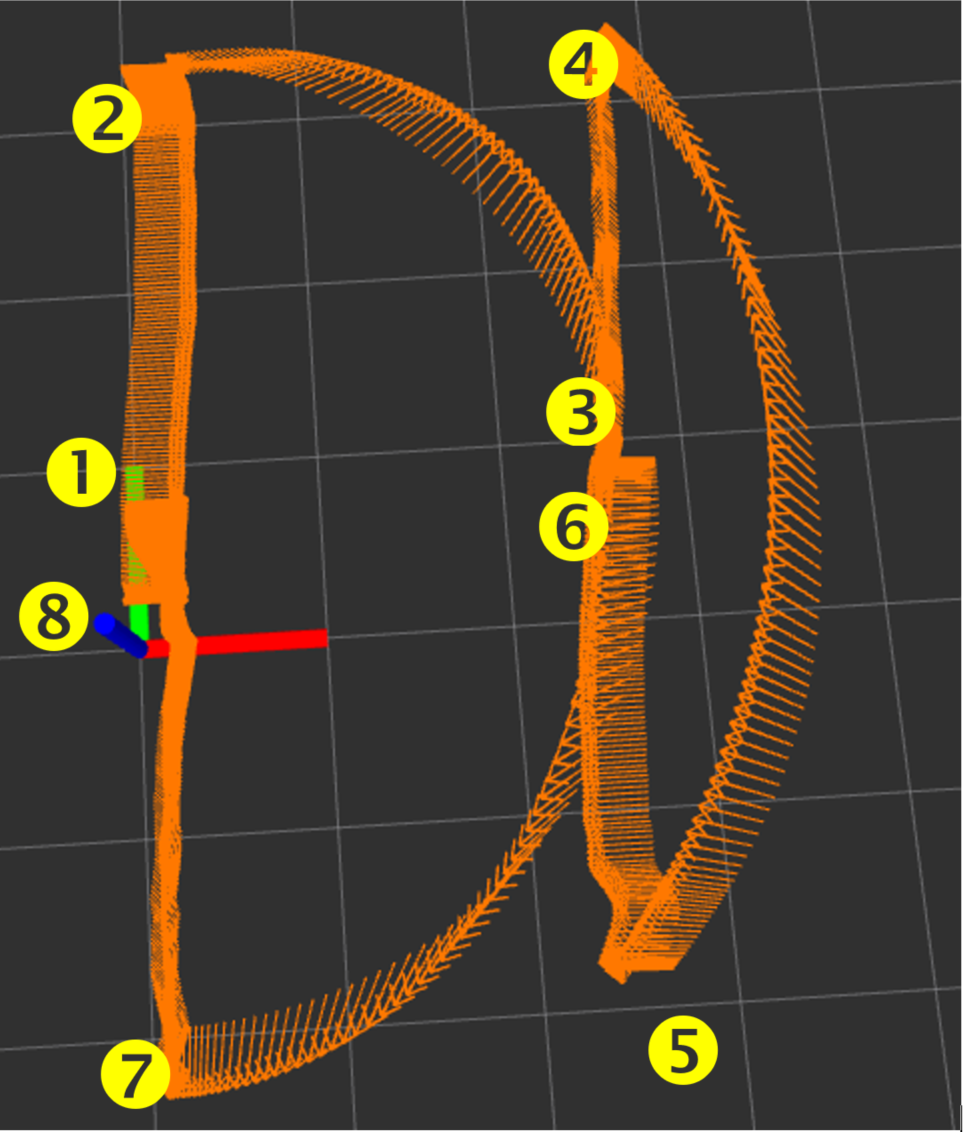
\includegraphics[width=0.4\textwidth]{rot_bug_rviz}
  \caption[Rviz Visualization of Rotational Distortion]{An Rviz visualization of PTAM's rotation defect. This image was created by moving the cart in a 3~m square pattern, turning 90\textdegree\ CCW at each corner.}
  \label{fig:rot_bug_rviz}
\end{wrapfigure}

Figure~\ref{fig:rot_bug_rviz} shows PTAM's susceptibility to losing tracking during rotation. This Rviz\footnote{A ROS visualization utility. \url{http://wiki.ros.org/rviz}} visualization was produced by moving the cart in a square trajectory and turning the cart by 90 degrees at each corner. The vehicle started at the origin (Point~1), then moved forward (in the $+y$ direction) in a straight line to Point~2. At Point~2, the cart was rotated counterclockwise in place by 90 degrees, producing the arc between Points~2 and 3. At this point, the cart was pointed in the $-x$ direction. As the figure shows, this arc extends \textit{opposite} the camera's true direction of travel. After rotating 90 degrees, the vehicle moved in a straight line in the $-x$ direction (Point~3 to Point~4), then rotated again by 90 degrees such that the cart was pointed in the $-y$ direction (Point~4 to 5). Again, the arc goes backward from the actual direction of travel, but this time its length is much greater. This was caused by rotating the vehicle at a higher speed than during the first turn, meaning that this rotation defect is velocity-dependent. From Point~5, the vehicle moves in the $-y$ direction to Point~6, rotates 90 degrees counterclockwise (Point~6 to 7), and then moves in a straight line back to a point near the origin (Point~8).

The trajectory plotted in Figure~\ref{fig:rot_bug_rviz} is vastly distorted. A trusting observer might surmise from the image that the vehicle moved in a pattern resembling two uppercase D's, as opposed to the square pattern traced out in reality. This rotation-translation bug in the ROS PTAM implementation is pervasive and prevents PTAM from being of any real use during rotation. For this reason, the experiments detailed in the next section were carefully performed without rotating the mobile test stand.

In other preliminary experiments, anomalous behavior was discovered in PTAM's $z$-position output. Over long translations, the vehicle's trajectory could be seen in

\begin{figure}[H]
  \centering
    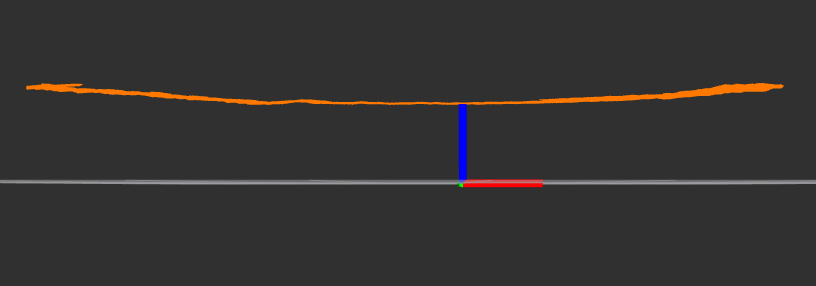
\includegraphics[width=\textwidth]{bowl-shaped_world}
  \caption[Rviz Visualization of Translational (Lens) Distortion]{An Rviz visualization of the ``bowl-shaped'' world seen by PTAM during a long translational motion. This image was created by translating the mobile test stand 3--4~meters in the $+x$ direction and then translating back 4--5~meters past the origin in the $-x$ direction.}
  \label{fig:bowl-shaped_world}
\end{figure}




\section{Experimental Procedures}
\todo{PTAM init process}
Two experiments were designed to characterize the UKF framework's effectiveness in various regimes of motion. The first experiment was a ``long walk'' in which the mobile test stand was translated in a straight line for several meters along the $y$-axis. This test was designed to characterize the effect of lens distortion in PTAM's output.

In the second experiment, the mobile test stand was moved in a rectangular ``box'' pattern at approximately constant speed, without rotation.

\begin{figure}[h]
  \centering
    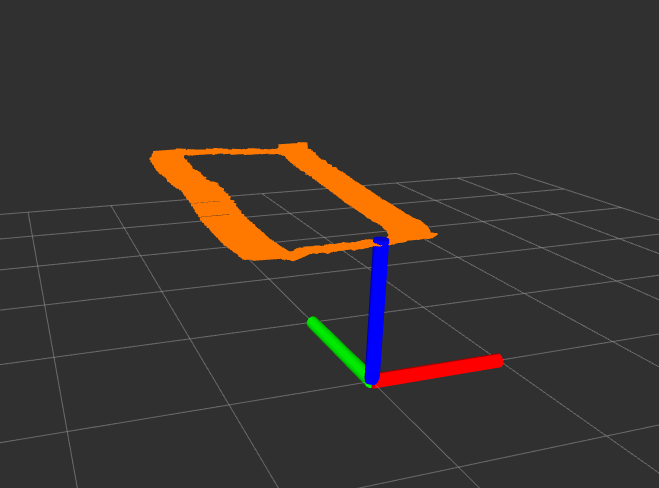
\includegraphics[width=\textwidth]{good_box_5_cropped}
  \caption[Rviz Visualization of a Box Pattern Trajectory]{An Rviz visualization of a box pattern trajectory. In this image, the orange segments are actually composed of arrows pointing along the vehicle's $x$-axis (parallel to the red axis at the origin). The experiment starts one meter above the origin and the mobile test stand is pushed in a rectangular pattern, coming to rest at the origin again.}
  \label{fig:good_box}
\end{figure}

\todo{describe each experiment}

Two data streams were collected for analysis using the \texttt{rosbag}\footnote{\url{http://wiki.ros.org/rosbag}} data recording utility.
\todo{more explanation of post processing}

\clearpage
\section{Materials}
\subsection{Computation and Sensing}
\begin{enumerate}
\item One (1) MatrixVision mvBlueFOX-MLC Camera\footnote{\url{https://www.matrix-vision.com/USB2.0-single-board-camera-mvbluefox-mlc.html}}
\item One (1) 1044\_0 PhidgetSpatial Precision 3/3/3 High Resolution IMU\footnote{\url{http://www.phidgets.com/products.php?product_id=1044}}
\item One (1) Hewlett-Packard Spectre x360 Convertible Laptop 13-ac076nr\footnote{\url{http://store.hp.com/us/en/pdp/hp-spectre-x360---13-ac076nr}}
\item Two (2) male Mini USB 2.0 to male USB Type A cables
\end{enumerate}
\subsection{Mobile Test Stand}
\begin{enumerate}
\item One (1) Oklahoma Sound PRC200 Premium Presentation Cart\footnote{\url{http://www.oklahomasound.com/products/product-category/single/?prod=9}}
\item One (1) 3D-printed Sensor Mount
\item Two (2) 4" C-Clamps
\item One (1) 1.2-meter 80/20\textsuperscript{\textregistered}~Inc.\ 1515 Rail\footnote{\url{https://8020.net/1515.html}}
\item One (1) 15 Series ``L'' Handle Linear Bearing Brake Kit\footnote{\url{https://8020.net/6800.html}}
\item One (1) $\frac{5}{16}$-18 $\times$ 0.687" Black FBHSCS (Screw)\footnote{\url{https://8020.net/shop/3320.html}}
\item Two (2) Slide-In Economy T-Nuts\footnote{Also available at \url{https://8020.net/shop/3320.html}}
\item Three (3) 1" Vicon Infrared Retroreflector Balls
\item Two (2) $\frac{1}{2}$" Vicon Infrared Retroreflector Balls
\item One (1) 0.7-meter Length of $\frac{1}{8}$"-thick Carbon Fiber Tube
\end{enumerate}
\pagebreak

\begin{figure}
  \centering
    \includegraphics[width=\textwidth]{cart_at_AI}
  \caption[Testing Environment]{The mobile test stand in the testing environment. The area shown is part of a larger motion capture facility. The floor is covered with rubber tiles, many of which bear April tags and QR codes for visual geometry.}
  \label{fig:cart_at_AI}
\end{figure}

\begin{figure}
  \centering
    \includegraphics[width=\textwidth]{sensor_mount_vicon}
  \caption[Sensor Mount Instrumented with Retroreflectors]{Close-up view of the sensor mount instrumented with Vicon infrared retroreflector balls.}
  \label{fig:sensor_mount_vicon}
\end{figure}